\subsection{Power Subsystem Testing}
\label{sec:power_subsystem_testing}
\paragraph{}The Power subsystem is an important part in making sure that the whole system is fully operational. With various components such as the microcontroller, sensors, mechanical components and more, we need to make sure that each component is operating properly. In this section we will test ways to see if the components are compatible with each other and function properly. This is a confirmation that the whole system is operating but also a test to see which parts work best with each other and what works best under given situations. One thing that will be tested is the voltage regulators to see which of the selected voltage regulators is most efficient and regulate power the best see fit.	\par
\subsubsection{Solar Panel Testing}
\paragraph{}The solar panels in the system are very important because they essentially collect all the power for the system to operate. We will be testing and verifying that the open circuit voltage and the operating current are what they are supposed to be outputing in direct sunlight. \par
This is a quite simple test only needing the solar panels and a multimeter. To test the voltage coming out of the solar panel,we will be place it outside and we will grab the multimeter and set higher than the voltage that is said on the solar panel. Connecting the multimeter to the ends of the solar panel we can confirm the voltage that the solar panel should be outputing. The same steps are done to test the current that should be outputed from the solar panels.\par
\begin{figure}[H]
    \centering
    \caption{Solar Panel Testing}
    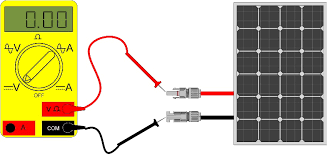
\includegraphics[width=\textwidth]{images/Solar_Panel_testing.png}
    \label{fig:Solar_Panel_testing}
\end{figure}
\subsubsection{Voltage Regulator}
\paragraph{}Providing power is an important part to operating a system, but providing the right amount of power is key to make sure all the components are operating properly. In this section we will test various designs from section 5 to see which of the designs for the given voltage regulators or from WEBENCH are best fit and most efficient. \par 
In this test, we will re-create the circuit designs that were in section 5, onto a breadboard using the right capacitors, resistors, and diodes. Then we will us an oscilloscope and a multimeter to measure the output voltages and currents for each design. This will help verify our theoretical values that we got from the design section in section 5. \par
As a resultant in the end, the outputs should be consistent with what we are looking for on the oscilloscope and the multimeter. After getting the final results from this test also, we can conclude which voltage regulator design we want to use for this system.\par